\documentclass[../main.tex]{subfiles}
En este capítulo se recogen las pruebas realizadas a la estación de tierra. A partir de los resultados obtenidos tanto en simulación como en pruebas reales se persigue su validación experimental. Estos experimentos han de comprobar que los objetivos descritos durante el Capítulo \ref{section:intro-objetivos} se cumplen. \\
En el momento de escribir esta sección, se han realizado dos pruebas de vuelo. Ambos experimentos con una aeronave de ala rotatoria, el 3DR Solo Drone (ver Figura \ref{fig:3dr}. La diferencia entre ellos es que uno se ha realizado con una misión polilínea mientras que el otro con una misión por patrón. Estos test de vuelo de la aplicación se verán con profundidad en las secciones de este capítulo. \\
Por último, y previo paso a las secciones con las pruebas de vuelo realizadas, se adjunta una lista de reproducción \footnote{https://www.youtube.com/playlist?list=PLGlX46StCA-QAXmeQp5omNhllGJ3CMjcO} que recoge la evolución de la aplicación a lo largo del tiempo con las distintas versiones realizadas. Aproximadamente cada mes se ha grabado un vídeo con las principales novedades de desarrollo durante ese periodo. Esta lista muestra una visión de las características de la aplicación y de los tiempos de desarrollo empleados.

\section{Prueba de vuelo para misiones polilínea.}
Este experimento reproduce un supuesto en el cual un operario realiza una misión polilínea \emph{in situ}, la envía a la aeronave y realiza el seguimiento de la misma. Para documentar la prueba de vuelo se ha generado un vídeo del que se adjunta su enlace \footnote{https://youtu.be/UOv8Go\_Q22k}. La Figura \ref{fig:prueba-pol} muestra un fotograma del vídeo mencionado. \\

La secuencia de ejecución seguida durante el experimento ha sido la siguiente:

\begin{enumerate}
    \item Ejecución de la aplicación y encendido del 3DR Solo junto a su emisora.
    \item Establecimiento de conexión entre ambos cuando el 3DR Solo ha establecido señal GPS (ver caso de uso \ref{subsection:results-caso4}).
    \item Caracterización de la aeronave y carga de pago (ver caso de uso \ref{subsection:results-caso1}). Este paso, pese haberlo realizado, resulta prescindible para las misiones polilínea.
    \item Creación de la misión polilínea (ver caso de uso \ref{subsection:results-caso3}).
    \item Validación de la misión creada.
    \item Comprobaciones pre-vuelo y envío de la misión a la aeronave.
    \item Inicio de la misión y seguimiento de la misma (ver caso de uso \ref{subsection:results-caso6}).
    \item Aterrizaje y fin de la misión.
\end{enumerate}

Es importante destacar que desde el momento de grabación del vídeo la aplicación ha seguido evolucionando y su versión actual es ligeramente diferente al momento del ensayo. Las diferencias son aspectos menores, pues las funcionalidades son prácticamente las mismas.

\begin{figure}[h]
    \centering
    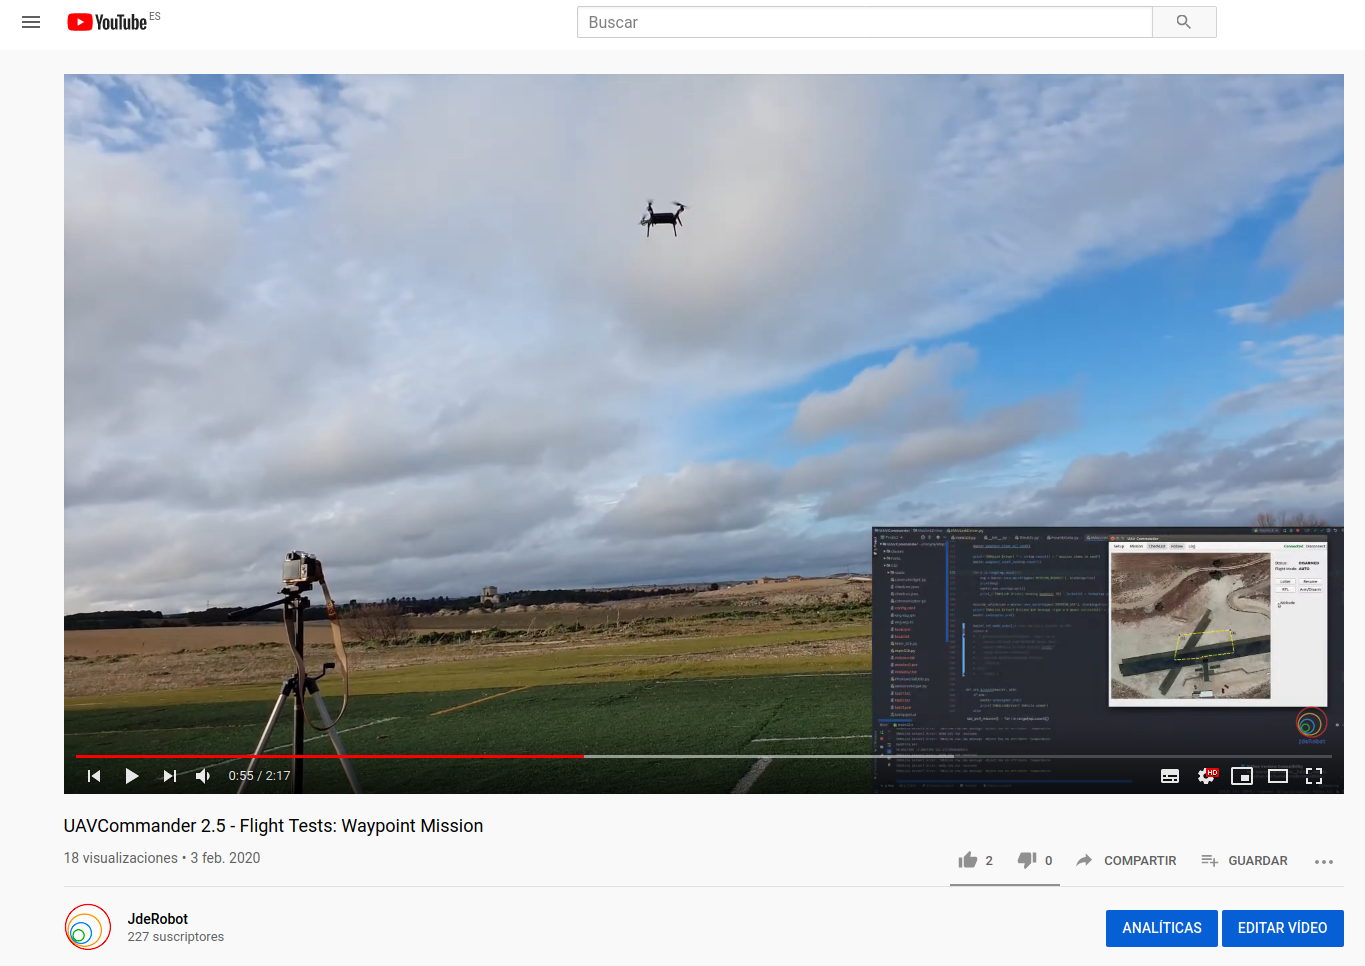
\includegraphics[width=0.9\textwidth]{prueba-pol.png}
    \caption{Vídeo con la prueba de vuelo para misiones polilínea.}
    \label{fig:prueba-pol}
\end{figure}

\section{Prueba de vuelo para misiones por patrón.}
Este ensayo de vuelo reproduce una situación en la cual un operario carga una misión por patrón previamente creada, la envía a la aeronave y realiza el seguimiento de la misma. Se adjunta un enlace de un vídeo \footnote{https://youtu.be/tpmpdkG0CjM} con el experimento real. Además, la Figura \ref{fig:prueba-pol} muestra un fotograma del vídeo adjunto. \\

La secuencia de ejecución seguida durante la prueba de vuelo ha sido la siguiente:

\begin{enumerate}
    \item Ejecución de la aplicación y encendido del 3DR Solo junto a su emisora.
    \item Establecimiento de conexión entre ambos cuando el 3DR Solo ha establecido señal GPS (ver caso de uso \ref{subsection:results-caso4}).
    \item Caracterización de la aeronave y carga de pago (ver caso de uso \ref{subsection:results-caso1}).
    \item Carga de una misión por patrón previamente confeccionada (ver caso de uso \ref{subsection:results-caso5}).
    \item Validación de la misión creada.
    \item Comprobaciones pre-vuelo y envío de la misión a la aeronave.
    \item Inicio de la misión y seguimiento de la misma (ver caso de uso \ref{subsection:results-caso6}).
    \item Aterrizaje y fin de la misión.
\end{enumerate}

Es importante destacar que algún aspecto menor del vídeo puede diferir con la versión actual, pues en el momento de grabación la aplicación se encontraba todavía en proceso de desarrollo.

\begin{figure}[h]
    \centering
    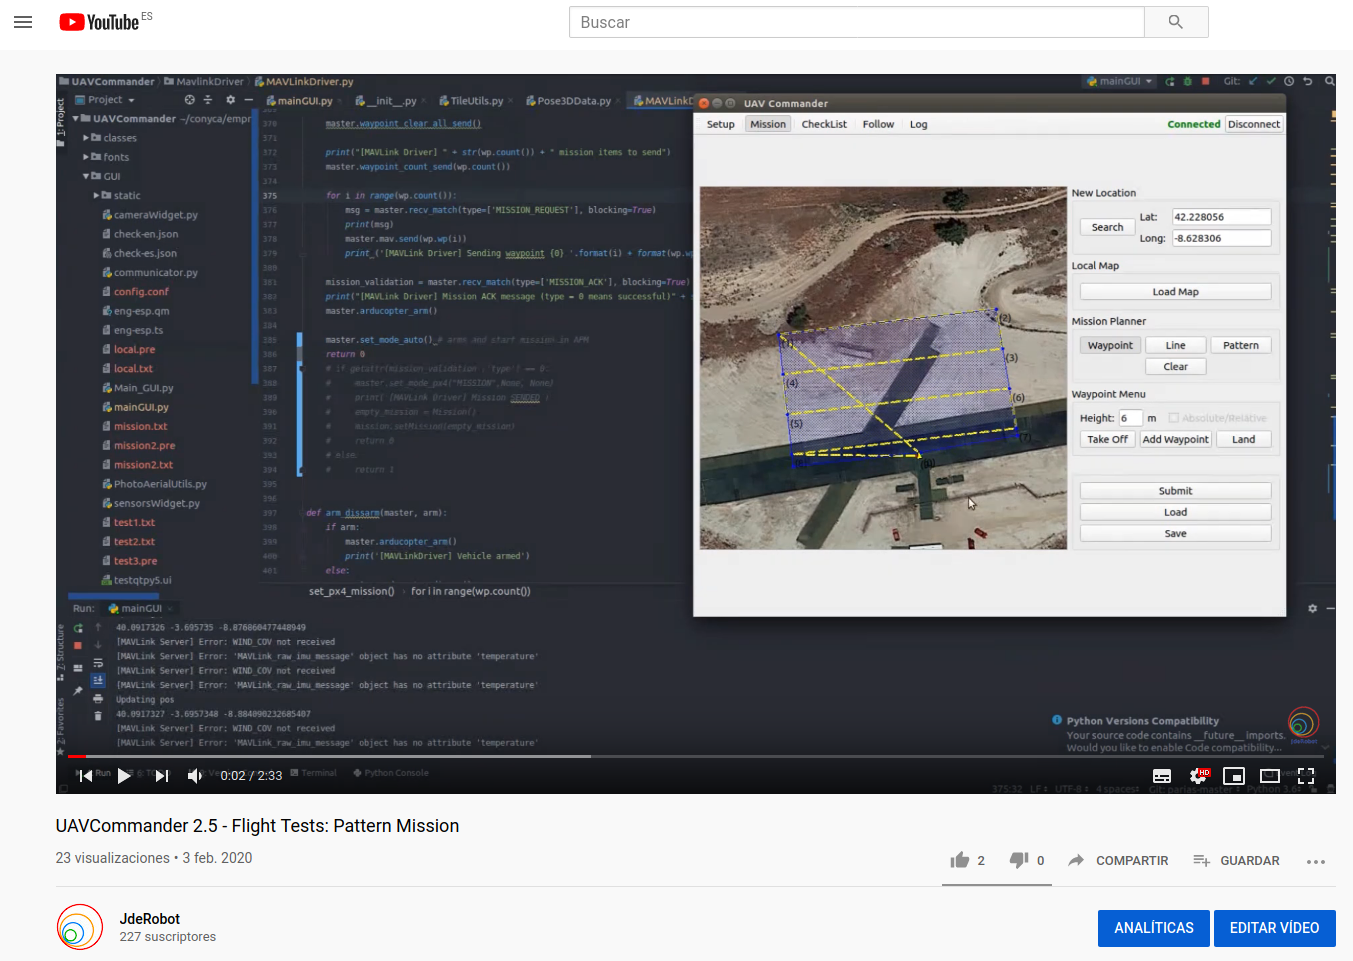
\includegraphics[width=0.9\textwidth]{prueba-patron.png}
    \caption{Vídeo con la prueba de vuelo para misiones por patrón.}
    \label{fig:prueba-patron}
\end{figure}